\chapter{Computo en GPU's}
Hasta hace 12 años la velocidad a la que crecían cada generación de procesadores era increíble, los programas eran tan rápidos como cada nueva generación de procesadores. Este crecimiento entre cada generación se detuvo, el problema es el consumo de energía y la disipación de calor, no permiten aumentar la frecuencia del reloj del procesador y el nivel de actividades por ciclo, en una sola unidad de procesamiento (CPU). Todos los productores de procesadores migraron a un nuevo modelo, los procesadores multinúcleo incrementaron el poder de procesamiento.

Este cambio en los procesadores tuvo un gran impacto a los programadores, la mayoría de las aplicaciones son escritas de forma secuencial,  por que la ejecución de estas son comprensibles paso a paso, mediante el código. Pero un programa secuencial ejecutándose en un solo núcleo del procesador, no sera más rápido. Entonces los programadores ya no pueden agregar cualidades y capacidades a sus programas.

Llega el momento de cambiar, si se desea que la calidad de los programas siga escalando con cada generación de procesadores, se deben crear programas que trabajen con múltiples hilos, cooperando todos para completar un trabajo mas rápido. Existen dos corrientes principales en cuanto a los procesadores multi-núcleo, el primero, es donde se pretende mantener la velocidad de los programas secuenciales, mientras se mueven entre múltiples núcleos; la segunda, se centra mas en la ejecución de aplicaciones en paralelo, tiene un gran numero de núcleos pequeños que va creciendo con cada generación. Es esta rama en la que entran las unidades de procesamiento gráfico o por sus siglas en ingles GPU.\cite{Kirk2010}

\section{GP-GPUs Nvidia}

"Las GPU han evolucionado al punto que muchas aplicaciones del mundo real se están implementando fácilmente en ellas y se ejecutan muchísimo más rápido que en sistemas con múltiples núcleos. Las arquitecturas de computación del futuro serán sistemas híbridos con GPU de núcleos paralelos trabajando en tándem con CPU de múltiples núcleos".\cite{GPUIntro}

\begin{figure}[h]
			\centering
				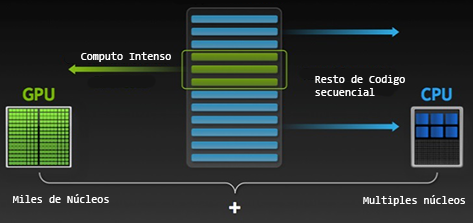
\includegraphics[scale=1]{img/how-gpu-acceleration-works.png}
			\caption{Sistema Híbrido}
\end{figure}

\subsection{Breve Historia}
La necesidad de mejores gráficos para los vídeo juegos, provocaron un gran avance en el hardware que se diseñaría. Desde principios de 1980 hasta finales de 1990 las tarjetas dedicadas a gráficos, no eran más que pipelines fijos que despliegan las formas geométricas calculadas por el CPU, por medio del hardware de acceso directo a memoria, por sus siglas en ingles DMA, esto les daba un funcionamiento fijo y apenas se podía configurar, con principalmente dos API, OpenGL de \textit{Silicon Graphics} y Direct3D de \textit{Microsoft}. Un ejemplo de estas tarjetas gráficas es, a la que se le acuño el nombre de GPU, la GeForce 256\cite{GeForce256} lanzada al mercado en 1999, aporta una capacidad visual sin precedentes, capaz de realizar las funciones de  transformación, iluminación, organización y rendering, con la capacidad de procesar 15 millones de triángulos por segundo y un rendimiento de 480 millones de píxeles por segundo. Su motor de rendering  256 bits muestra una mejora en cuanto a la complejidad visual.

Toda esta tecnología tan revolucionaria llamo la atención de otros profesionales, que se integraron a el trabajo de los artistas y desarrolladores de vídeo juegos, utilizando el gran rendimiento de punto flotante que tenían los GPU para otros objetivos. De esta forma surge el movimiento de la GPU para fines generales(GP-GPU).

Pero en ese momento, la GP-GPU era muy difícil de manipular, solo aquellos que tenían amplios conocimientos en lenguajes de programación de gráficos, desarrollaban para esta plataforma. Pero aun que memorizaras el API entera se enfrentaba un reto, donde los cálculos para resolver problemas generales debían ser representados por triángulos o polígonos.

Fue hasta 2001, en la Universidad de Stanford un equipo, liderado por Ian Buck, que se propuso ver el GPU como un  \textit{procesador de flujos}. Este equipo desarrollaría \textit{Brook} \cite{Buck2001}, un lenguaje de programación diseñado para ser igual a la sintaxis de C, con algunas características adicionales. El lenguaje se desarrolla con el objetivo de minimizar el complejo trabajo de análisis, que se requería para generar aplicaciones paralelas. Introducirían conceptos como los flujos(streams), kernels y los operadores de reducción. Todo esto le dio un gran impulso a los GPU como procesadores de propósitos generales, ya que el lenguaje era mas fácil de manejar, ya que era de más alto nivel, y lo mas importante los programas escritos en \textit{Brook} eran hasta 7 veces mas rápido que códigos similares existentes.

La compañía NVIDIA se dio cuenta que tenia un hardware muy poderoso en las manos, pero debía complementarlo con herramientas de hardware y software intuitivas, con ello le hicieron la invitación a Ian Buck para colaborar con ellos, el objetivo sería ejecutar C a la perfección en una GPU. NVIDIA alcanza este objetivo en 2006 con el lanzamiento de CUDA, la cual seria la primera solución para las GP-GPU, y aunado a esta solución, lanza la GeForce 8800 la cual fue diseñada, para ser usada en cómputo de propósito general, y su arquitectura fue pensada en la de CUDA. 

\section{CUDA}
Compute Unified Device Architecture (CUDA) es una plataforma para computo paralelo y un modelo de programación, que NVIDIA lanzo en noviembre de 2006, permitiendo obtener aumentos en los rendimientos del computo, esto es gracias a la ayuda que la unidad de procesamiento de gráficos, le proporciona al CPU. 

Los dispositivos CUDA aceleran la ejecución de los programas que tienen una gran cantidad de datos a procesar, ya que la arquitectura de esta plataforma, de la cual se hablara adelante, es como un procesador tradicional como el que las computadoras tienen, solo que tienen la cualidad de que los procesadores son masivamente paralelos equipados con una gran cantidad de unidades aritméticas. En las cuales se ejecutara la misma instrucción en todas, respecto a la taxonomía de Flynn, la categoría seria de \textit{una instrucción, multiples datos} (SIMD). 

\begin{figure}[h]
			\centering
				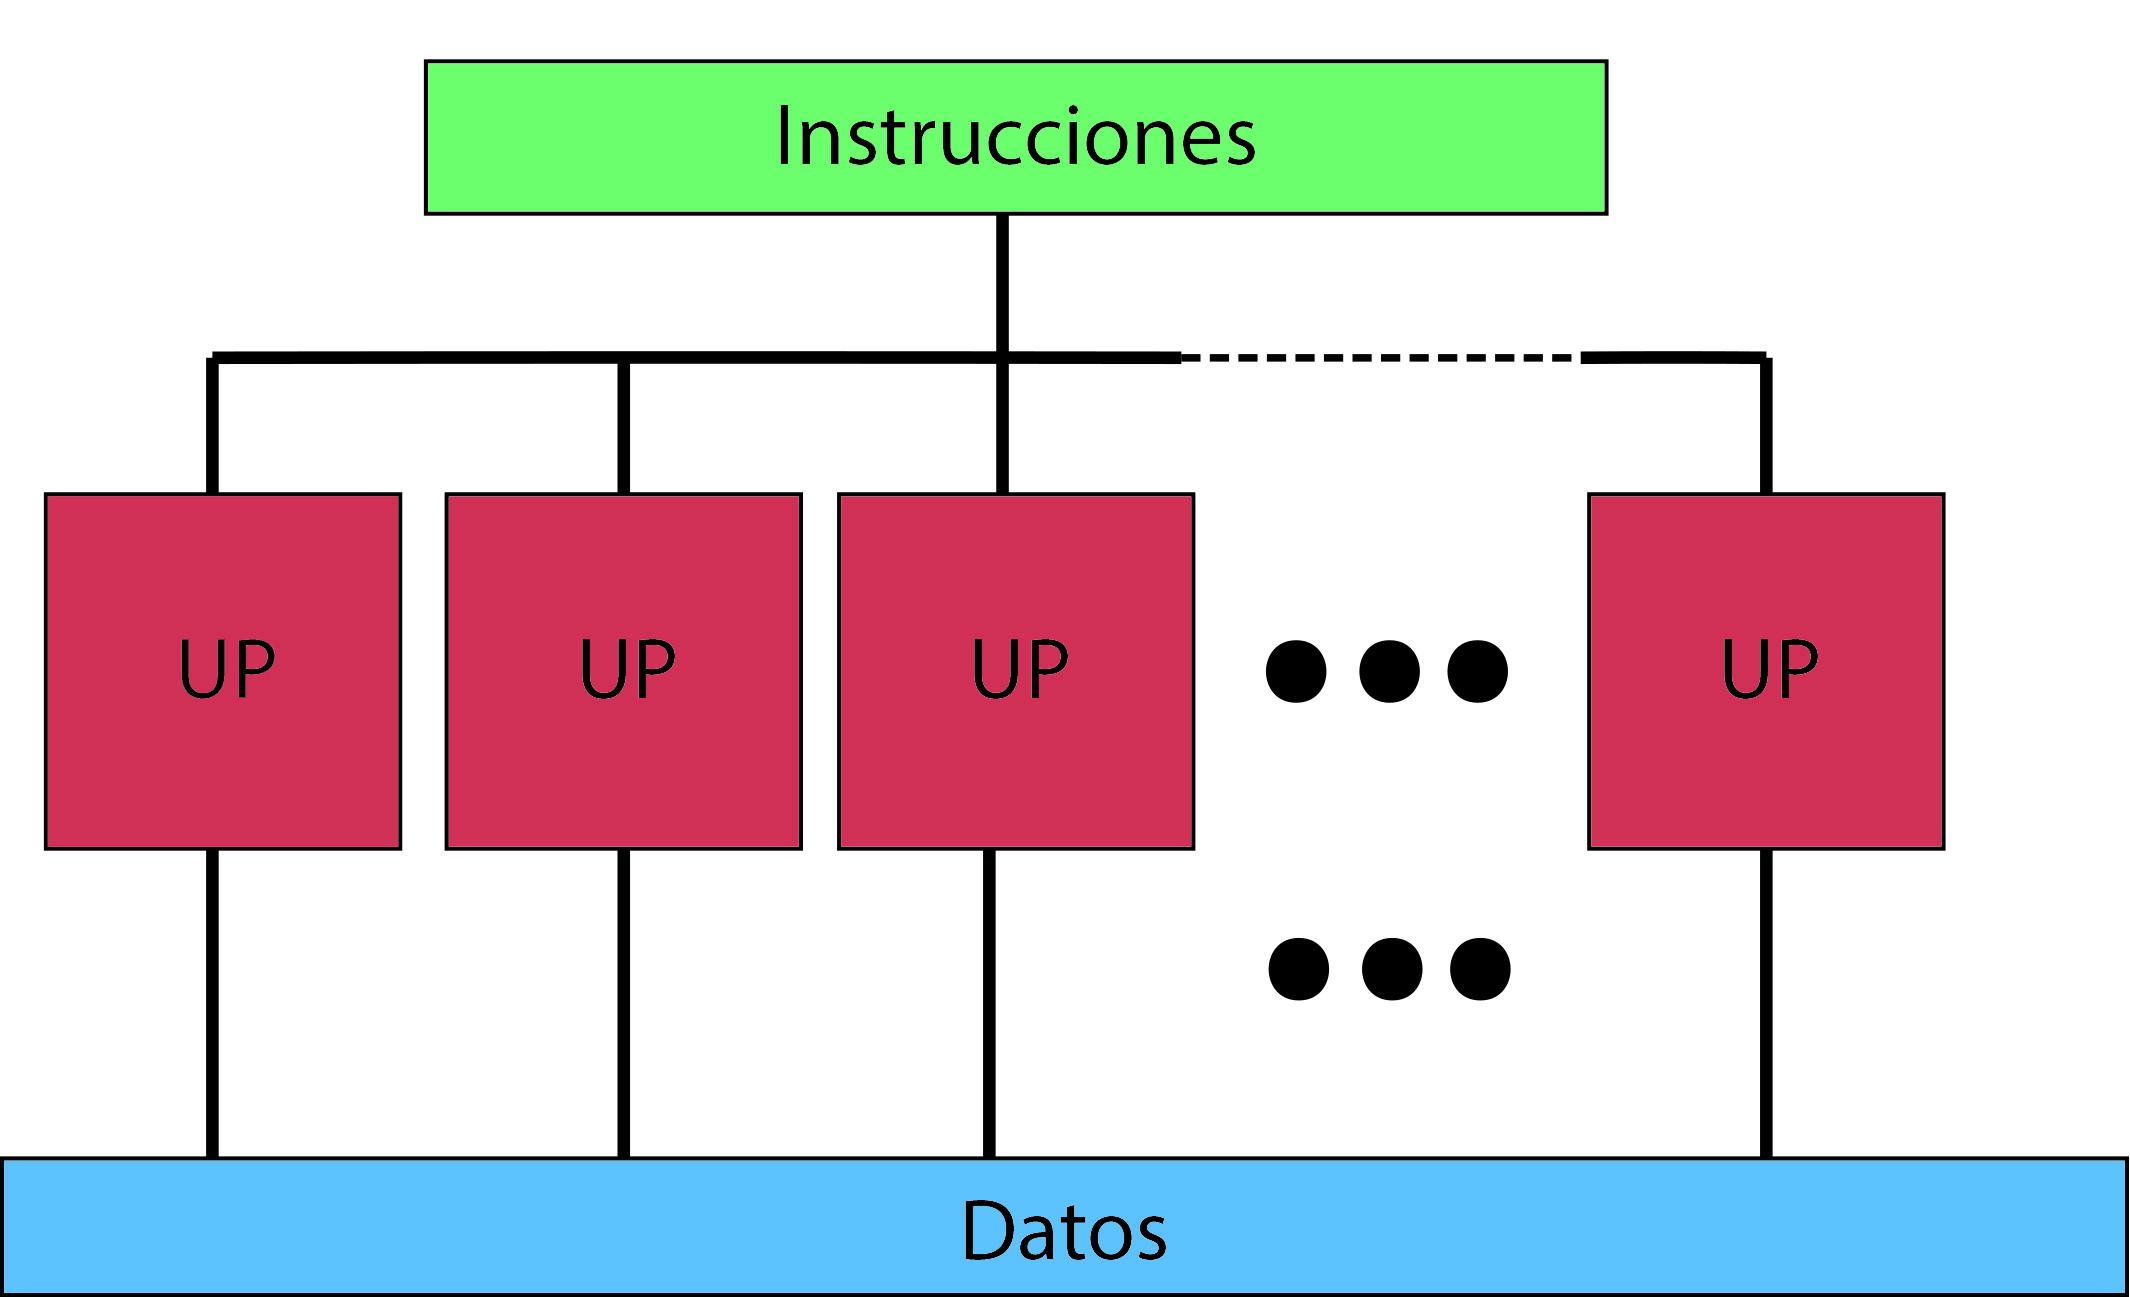
\includegraphics[scale=0.2]{img/SIMD.jpg}
			\caption{SIMD}
\end{figure}


Respecto al modelo de programación para desarrollar los programas para las GPU, es gracias a una extensión del lenguaje C, conocida como CUDA C. Existen alternativas a esta extensión, se pueden utilizar lenguajes como FORTRAN, Python, .NET combinando CUDA con Microsoft's F\# o alguna API como OpenCL u OpenACC\cite{lenguajes}. 
 

\subsection{Arquitecturas}
La arquitectura de CUDA fue diseñada, para que la GPU pudiera ser utilizada en aplicaciones de propósito general. En la cual se tiene un arreglo de procesadores con múltiples unidades aritmético lógica, por sus siglas en ingles ALU, las cuales para alcanzar este objetivo, fueron diseñadas para poder realizar operaciones de punto flotante, cumpliendo los requisitos del Instituto de Ingeniería Eléctrica y Electrónica (IEEE). Aparte de esto las ALU debían tener acceso a diferentes tipos de memoria, como la compartida entre unidades y la memoria de la tarjeta gráfica. 

Estas ALU tan particulares, en la arquitectura de CUDA las conoceremos como \textit{CUDA cores}, conforman gran parte de los Streaming Multiprocessor (SM). Los SM son procesadores que tienen la tarea de ejecutar los hilos concurrentemente, aparte de los CUDA cores tienen, están formados por una memoria cache(shared memory), registros y algunas unidades de funciones especiales.

\subsubsection{Fermi}

Los GPU basados en la arquitectura Fermi, están formados por 512 CUDA cores. Los CUDA cores ejecutan operaciones de punto flotantes o enteras por ciclo de reloj, y por cada uno de los hilos. Los 512 CUDA cores están organizados en 16 SM de 32 cores cada uno. El GPU tiene seis particiones de memoria de 64-bits, capacidad para leer 384-bits de la memoria simultáneamente y con una capacidad de hasta 6GB de memoria DRAM categoría DDR5. El sistema de conexión entre el GPU y el CPU es vía PCI-Express.






\subsection{Modelo de Programación}
\subsection{Rendimiento}

